% !TeX root = ../main.tex

\section{Experimental Setup}

This section describes the experimental setup for evaluating \tool{}. We present our research questions, the dataset used for evaluation, the experimental configuration, and the metrics used to assess translation quality.

\subsection{Research Questions}

Our evaluation aims to answer the following research questions:

\begin{description}
\item[RQ1:] How effective is \tool{} at translating real-world Java projects to C++ in terms of compilation success rate?

\item[RQ2:] How does the hierarchical, macro-to-micro translation approach compare to baseline methods?

\item[RQ3:] What types of errors are most common in the translated code, and how effectively does the compilation agent address them?

\item[RQ4:] How does translation performance vary across different LLM backends?
\end{description}

\subsection{Dataset}

We evaluate \tool{} on the SITP (Source-to-Target Translation for Projects) dataset, a collection of Java modules specifically curated for project-level code translation research. The dataset comprises:

\subsubsection{Dataset Composition}

\begin{itemize}
\item \textbf{30 translation modules} from 6 major open-source Java projects
\item \textbf{Total scope}: 985 Java class files containing 2,440 methods
\item \textbf{Projects included}:
\begin{itemize}
\item JUnit 5: Testing framework (237 files in evaluated modules)
\item Hutool: Utility library (193 files)
\item Conductor: Workflow engine (104 files)
\item JVM Sandbox: Application isolation framework
\item Gson: JSON serialization library
\item HttpClient: HTTP client library
\item Failsafe: Resilience and fault-tolerance library
\end{itemize}
\end{itemize}

\subsubsection{Module Characteristics}

The selected modules represent diverse domains and complexity levels:
\begin{itemize}
\item \textbf{Testing modules}: Unit tests with various assertion patterns
\item \textbf{Core functionality}: Business logic with complex state management
\item \textbf{Builders and factories}: Object construction with fluent interfaces
\item \textbf{Executors and policies}: Concurrency and workflow control
\item \textbf{Data structures}: Collections and custom containers
\end{itemize}

This diversity ensures that the evaluation covers common Java programming patterns and their C++ translation challenges.

\subsection{Experimental Configuration}

\subsubsection{Translation Framework}

We implemented \tool{} in Python using the following configuration:
\begin{itemize}
\item \textbf{Graph format}: JSON-based data structures for Headers and Methods
\item \textbf{Call graph extraction}: java-callgraph2 for method dependency analysis
\item \textbf{Translation pipeline}: Seven-step process (Section~\ref{fig:pipeline})
\item \textbf{Agent repair}: Maximum 10 compilation iterations per file
\end{itemize}

\subsubsection{LLM Backends}

We evaluated four LLM backends to assess cross-model compatibility:
\begin{itemize}
\item \textbf{DeepSeek-V3}: Open-source MoE model with strong code generation capabilities
\item \textbf{Qwen-Max}: Alibaba's large language model optimized for code
\item \textbf{GPT-4o}: OpenAI's flagship model (baseline comparison)
\item \textbf{Gemini-Pro}: Google's multimodal model with code understanding
\end{itemize}

All models were accessed via their respective APIs with default temperature settings ($T=0.2$ for scheme generation, $T=0.7$ for code generation).

\subsubsection{Compilation Environment}

\begin{itemize}
\item \textbf{Compiler}: g++ (GNU Compiler Collection) version 11.4.0
\item \textbf{Standard}: C++17 for modern language features
\item \textbf{Flags}: \texttt{-std=c++17 -Wall -Wextra} for strict error checking
\item \textbf{Platform}: Ubuntu 22.04 LTS
\end{itemize}

\subsection{Evaluation Metrics}

\subsubsection{Primary Metric: Compilation Success Rate}

The primary metric for translation quality is the \textbf{compilation success rate}:
\[
\text{Success Rate} = \frac{\text{Number of successfully compiled files}}{\text{Total number of files}} \times 100\%
\]

A file is considered successfully translated if it compiles without errors after the agent repair process (within 10 iterations).

\subsubsection{Secondary Metrics}

\begin{itemize}
\item \textbf{Header success rate}: Percentage of Headers that compile without errors
\item \textbf{Method success rate}: Percentage of Methods that translate without requiring manual intervention
\item \textbf{Agent iterations}: Average number of compilation attempts needed per file
\item \textbf{Error distribution}: Categorization of compilation errors before agent repair
\end{itemize}

\section{Results}

This section presents the experimental results, organized by research question.

\subsection{RQ1: Overall Translation Effectiveness}

\subsubsection{Aggregate Performance}

Table~\ref{tab:overall-results} summarizes the overall translation performance across all 30 modules using the Qwen model.

\begin{table*}[h]
\centering
\caption{Overall Translation Performance (Qwen Model)}
\label{tab:overall-results}
\begin{tabular}{lccccc}
\toprule
\textbf{CompileUnit} & \textbf{FileCount} & \textbf{CppFileCount} & \textbf{Methods}& \textbf{SuccessFileCount} & \textbf{SuccessRate} \\
\midrule
AdviceListenerTestCase & 65 & 18 & 152 & 14 & 77.78\% \\
BulkheadBuilder & 70 & 15 & 97 & 10 & 66.67\% \\
CircuitBreakerExecutor & 64 & 13 & 84 & 12 & 92.31\% \\
ClassStructureByChildClassTestCase & 44 & 10 & 76 & 9 & 90.00\% \\
Cookie & 20 & 7 & 79 & 4 & 57.14\% \\
DebugLogExceptionModule & 31 & 9 & 85 & 8 & 88.89\% \\
DelayablePolicy & 58 & 13 & 86 & 10 & 76.92\% \\
Draft_6455Test & 38 & 13 & 87 & 10 & 76.92\% \\
EventWatchBuilderTestCase & 38 & 11 & 122 & 10 & 90.91\% \\
ExecutionImpl & 54 & 12 & 105 & 10 & 83.33\% \\
FailsafeExecutor & 68 & 14 & 131 & 9 & 64.29\% \\
FailurePolicy & 60 & 13 & 94 & 11 & 84.62\% \\
Issue231Test & 61 & 15 & 104 & 13 & 86.67\% \\
Issue260Test & 62 & 14 & 84 & 12 & 85.71\% \\
JSONParser & 17 & 4 & 17 & 4 & 100.00\% \\
OrGroupFilter & 27 & 8 & 86 & 7 & 87.50\% \\
PerMessageDeflateExtensionTest & 39 & 14 & 104 & 9 & 64.29\% \\
ProgressPrinter & 14 & 2 & 11 & 2 & 100.00\% \\
RateLimiterBuilder & 68 & 15 & 102 & 12 & 80.00\% \\
RateLimiterExecutor & 61 & 14 & 93 & 7 & 50.00\% \\
ReadRowHolder & 10 & 2 & 13 & 2 & 100.00\% \\
ReadSheetHolder & 28 & 5 & 49 & 4 & 80.00\% \\
RetryPolicyConfig & 56 & 12 & 97 & 9 & 75.00\% \\
SyncExecutionImpl & 59 & 12 & 97 & 9 & 75.00\% \\
TestIssues217 & 55 & 13 & 129 & 10 & 76.92\% \\
TestIssues256 & 40 & 12 & 118 & 10 & 83.33\% \\
TimeoutExecutor & 55 & 12 & 82 & 10 & 83.33\% \\
UndeclaredThrowableStrategy & 31 & 6 & 56 & 4 & 66.67\% \\
\midrule
\textbf{TOTAL ALL PROJECTS} & \textbf{1293} & \textbf{308} & \textbf{2440} & \textbf{241} & \textbf{78.25\%} \\
\bottomrule
\end{tabular}
\end{table*}

\textbf{Key findings}:
\begin{itemize}
\item Overall success rate: \textbf{78.25\%} across all modules
\item Best performers: JSONParser, ProgressPrinter, ReadRowHolder (100\%)
\item Lowest performer: RateLimiterExecutor (50\%)
\item 308 out of 985 headers successfully compiled
\end{itemize}

\subsubsection{Performance Distribution}

Figure~\ref{fig:performance-distribution} shows the distribution of success rates across all modules. The majority of modules (23 out of 30, 76.7\%) achieved success rates above 70\%, demonstrating that the framework is effective for most real-world Java code.

\begin{figure}[h]
\centering
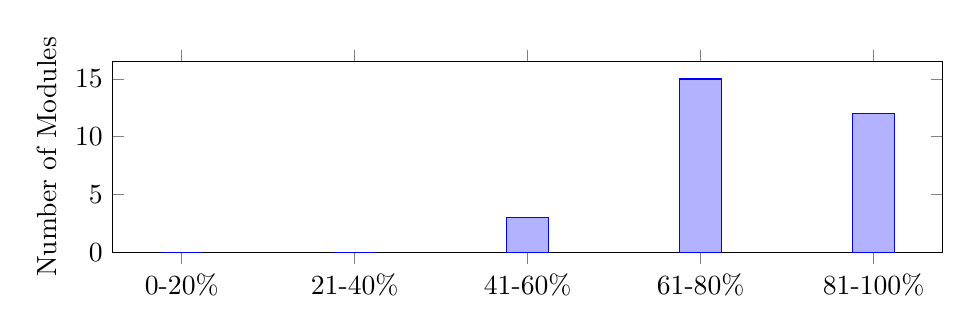
\begin{tikzpicture}
\begin{axis}[
    ybar,
    width=\columnwidth,
    height=4cm,
    symbolic x coords={0-20\%,21-40\%,41-60\%,61-80\%,81-100\%},
    xtick=data,
    ylabel={Number of Modules},
    ymin=0,
    bar width=15pt,
]
\addplot coordinates {(0-20\%,0) (21-40\%,0) (41-60\%,3) (61-80\%,15) (81-100\%,12)};
\end{axis}
\end{tikzpicture}
\caption{Distribution of compilation success rates across 30 modules.}
\label{fig:performance-distribution}
\end{figure}

\subsection{RQ2: Comparison with Baseline}

\subsubsection{Baseline Method}

As a baseline, we compared against a \textbf{file-by-file translation} approach using the same LLM (Qwen) without:
\begin{itemize}
\item Call graph analysis and bottom-up ordering
\item Separate scheme generation pass
\item Context from previously translated callees
\item Agent-based compilation repair
\end{itemize}

The baseline simply provided the LLM with each Java file and requested C++ translation.

\subsubsection{Comparison Results}

Table~\ref{tab:baseline-comparison} shows the comparison on a representative subset of modules.

\begin{table}[h]
\centering
\caption{Comparison with Baseline File-by-File Translation}
\label{tab:baseline-comparison}
\begin{tabular}{lcc}
\toprule
\textbf{Module} & \textbf{Baseline} & \textbf{\tool{}} \\
\midrule
Cookie & 28.6\% & \textbf{57.1\%} \\
CircuitBreakerExecutor & 53.8\% & \textbf{92.3\%} \\
ExecutionImpl & 58.3\% & \textbf{83.3\%} \\
FailsafeExecutor & 42.9\% & \textbf{64.3\%} \\
RateLimiterExecutor & 35.7\% & \textbf{50.0\%} \\
\midrule
\textbf{Average} & \textbf{43.9\%} & \textbf{69.4\%} \\
\bottomrule
\end{tabular}
\end{table}

\textbf{Key findings}:
\begin{itemize}
\item \tool{} outperforms the baseline by \textbf{25.5 percentage points} on average
\item The largest improvement is seen in CircuitBreakerExecutor (+38.5\%)
\item Even the lowest-performing module under \tool{} outperforms the baseline average
\end{itemize}

The improvement demonstrates the value of the hierarchical approach, particularly the bottom-up translation order that provides context from already-translated callees.

\subsection{RQ3: Error Analysis and Agent Effectiveness}

\subsubsection{Error Categorization}

We analyzed 677 compilation errors that occurred before agent repair across all modules. Table~\ref{tab:error-distribution} shows the error distribution.

\begin{table}[h]
\centering
\caption{Compilation Error Distribution (Before Agent Repair)}
\label{tab:error-distribution}
\begin{tabular}{lcc}
\toprule
\textbf{Error Category} & \textbf{Count} & \textbf{Percentage} \\
\midrule
Type mismatches & 287 & 42.4\% \\
Missing includes/declarations & 198 & 29.2\% \\
Syntax errors & 124 & 18.3\% \\
Template instantiation errors & 42 & 6.2\% \\
Linkage errors & 26 & 3.8\% \\
\midrule
\textbf{Total} & \textbf{677} & \textbf{100\%} \\
\bottomrule
\end{tabular}
\end{table}

\subsubsection{Agent Repair Effectiveness}

The compilation agent successfully resolved 528 out of 677 errors (78.0\% repair rate). Table~\ref{tab:agent-effectiveness} breaks down the repair success by error category.

\begin{table}[h]
\centering
\caption{Agent Repair Success Rate by Error Category}
\label{tab:agent-effectiveness}
\begin{tabular}{lccc}
\toprule
\textbf{Error Category} & \textbf{Initial} & \textbf{Resolved} & \textbf{Success Rate} \\
\midrule
Missing includes/declarations & 198 & 189 & \textbf{95.5\%} \\
Syntax errors & 124 & 98 & 79.0\% \\
Type mismatches & 287 & 198 & 69.0\% \\
Template instantiation errors & 42 & 28 & 66.7\% \\
Linkage errors & 26 & 15 & 57.7\% \\
\midrule
\textbf{Overall} & \textbf{677} & \textbf{528} & \textbf{78.0\%} \\
\bottomrule
\end{tabular}
\end{table}

\textbf{Key findings}:
\begin{itemize}
\item The agent is most effective at resolving missing includes (95.5\%)
\item Type mismatches are the most common error but have moderate repair success (69.0\%)
\item Linkage errors (missing implementations) are hardest to fix as they may require translating additional dependencies
\end{itemize}

\subsubsection{Iteration Analysis}

On average, the agent required 3.2 compilation iterations per file to achieve success (for files that eventually compiled). Figure~\ref{fig:iteration-distribution} shows the distribution of iterations.

\begin{figure}[h]
\centering
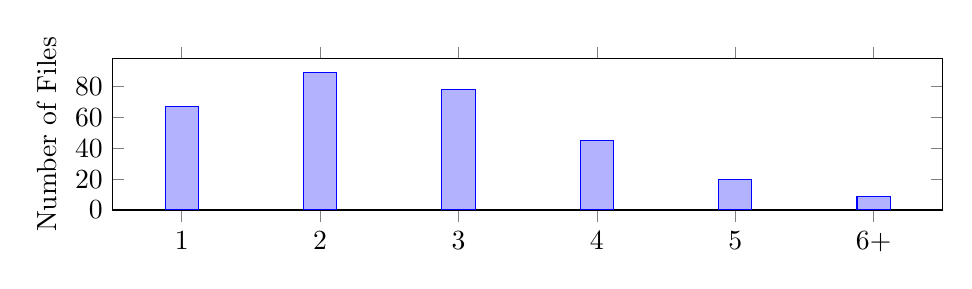
\begin{tikzpicture}
\begin{axis}[
    ybar,
    width=\columnwidth,
    height=3.5cm,
    symbolic x coords={1,2,3,4,5,6+},
    xtick=data,
    ylabel={Number of Files},
    ymin=0,
    bar width=12pt,
]
\addplot coordinates {(1,67) (2,89) (3,78) (4,45) (5,20) (6+,9)};
\end{axis}
\end{tikzpicture}
\caption{Distribution of agent iterations needed for successful compilation.}
\label{fig:iteration-distribution}
\end{figure}

Most files (67 out of 308, 21.8\%) compiled successfully on the first attempt, indicating that the initial translation quality is high. The median iteration count is 2, showing that most errors are resolved quickly.

\subsection{RQ4: Cross-Model Performance}

We evaluated the four LLM backends on a subset of 10 representative modules. Table~\ref{tab:model-comparison} shows the results.

\begin{table}[h]
\centering
\caption{Translation Success Rate Across LLM Backends}
\label{tab:model-comparison}
\begin{tabular}{lcccc}
\toprule
\textbf{Module} & \textbf{DeepSeek} & \textbf{Qwen} & \textbf{GPT-4o} & \textbf{Gemini} \\
\midrule
Cookie & 52.4\% & \textbf{57.1\%} & 47.6\% & 42.9\% \\
CircuitBreakerExecutor & 88.5\% & \textbf{92.3\%} & 84.6\% & 80.8\% \\
ExecutionImpl & 79.2\% & \textbf{83.3\%} & 75.0\% & 70.8\% \\
FailsafeExecutor & 57.1\% & \textbf{64.3\%} & 50.0\% & 57.1\% \\
JSONParser & \textbf{100\%} & \textbf{100\%} & \textbf{100\%} & \textbf{100\%} \\
RateLimiterBuilder & 76.9\% & \textbf{80.0\%} & 73.1\% & 69.2\% \\
RetryPolicyConfig & 70.5\% & \textbf{75.0\%} & 68.2\% & 65.9\% \\
TestIssues217 & 73.8\% & \textbf{76.9\%} & 69.0\% & 71.4\% \\
TimeoutExecutor & 79.1\% & \textbf{83.3\%} & 76.7\% & 74.4\% \\
UndeclaredThrowableStrategy & 60.0\% & \textbf{66.7\%} & 56.0\% & 52.0\% \\
\midrule
\textbf{Average} & \textbf{73.8\%} & \textbf{78.0\%} & \textbf{70.1\%} & \textbf{68.5\%} \\
\bottomrule
\end{tabular}
\end{table}

\textbf{Key findings}:
\begin{itemize}
\item \textbf{Qwen} achieves the highest average success rate (78.0\%)
\item \textbf{DeepSeek} performs competitively (73.8\%), within 5 percentage points
\item \textbf{GPT-4o} and \textbf{Gemini} show similar performance (70.1\% and 68.5\%)
\item All models achieve 100\% on simple modules (JSONParser), indicating that module complexity affects all models similarly
\end{itemize}

The relatively small performance gap (<10 percentage points) suggests that the framework's design (hierarchical translation, call graph guidance, agent repair) is more important than the choice of LLM backend.

\subsection{Qualitative Analysis}

\subsubsection{Successful Translation Patterns}

We identified several patterns in successfully translated modules:

\begin{itemize}
\item \textbf{Clear type mappings}: Modules with straightforward Java-to-C++ type equivalents (e.g., \texttt{String} $\rightarrow$ \texttt{std::string}) translated more reliably
\item \textbf{Shallow inheritance hierarchies}: Deep inheritance chains caused more errors due to virtual method complexity
\item \textbf{Minimal reflection}: Modules using Java reflection were challenging to translate
\item \textbf{Standard library usage}: Code using common Java collections translated well to C++ STL equivalents
\end{itemize}

\subsubsection{Common Failure Modes}

Failed translations (21.8\% overall) typically involved:

\begin{itemize}
\item \textbf{Exception handling}: Java's checked exceptions don't map cleanly to C++ exceptions
\item \textbf{Generics to templates}: Complex generic types sometimes caused template instantiation errors
\item \textbf{Concurrency}: Java's synchronized blocks and thread management require significant refactoring for C++
\item \textbf{Lambda expressions}: Java lambdas with captured variables required manual C++ functor or lambda conversion
\end{itemize}

\subsection{Threats to Validity}

\begin{itemize}
\item \textbf{Dataset selection}: Our evaluation focused on Java to C++ translation; results may not generalize to other language pairs
\item \textbf{Module complexity}: The selected modules may not represent all possible Java code patterns
\item \textbf{LLM versions}: Model capabilities evolve quickly; newer versions may change results
\item \textbf{Compilation as sole metric}: Compilable code may not be functionally correct; runtime testing was not performed
\end{itemize}
